
\documentclass[aspectratio=169]{beamer}
%[handout]

\usetheme[progressbar=frametitle]{metropolis}
\usepackage{appendixnumberbeamer}

\usepackage[utf8]{inputenc}
\usepackage[T1]{fontenc}

\usepackage[brazil]{babel}
\usepackage[outputdir=..]{minted}
\usepackage{xcolor}
\usepackage{soul} % strikethrough
\usepackage{advdate}
\usepackage{graphicx}
\graphicspath{{figs/}}
\usepackage{graphbox}

\usepackage[ampersand]{easylist}

\usepackage{multirow}
\usepackage{multicol}
\usepackage{subcaption}

\usepackage{pgf,tikz}
\usetikzlibrary{shapes,arrows,positioning}
\usetikzlibrary{circuits.logic.US}
\usetikzlibrary{matrix,calc}

\usepackage{karnaugh-map}

\usepackage{pgfpages}
\setbeameroption{hide notes} % Only slides
% \setbeameroption{show only notes} % Only notes
% \setbeameroption{show notes on second screen=right} % Both

% \graphicspath{{../figs/}}

\definecolor{bgc}{rgb}{0.95,0.9,0.95}
\definecolor{links}{HTML}{2A7F7F}
\hypersetup{colorlinks,linkcolor=,urlcolor=links}

\newminted{verilog}{fontsize=\scriptsize, 
    linenos,
    numbersep=8pt,
    bgcolor=bgc,
    tabsize=4,
    framesep=3mm} 
    %frame=lines,

\newcommand{\verilog}[1]{\verilogf{#1}{\footnotesize}}

\newcommand{\verilogf}[2]{\inputminted[fontsize=#2, 
    linenos,
    tabsize=2,
    numbersep=4pt,
    bgcolor=bgc,
    framesep=3mm]{verilog}{../codes/#1.v}
}

\newminted{nasm}{fontsize=\scriptsize, 
		   linenos,
		   numbersep=8pt,
           bgcolor=bgc,
		   framesep=3mm} 

\usepackage{booktabs}
\usepackage[scale=2]{ccicons}

\usepackage{pgfplots}
\usepgfplotslibrary{dateplot}

\usepackage{hyperref}


\usepackage{xspace}
\newcommand{\themename}{\textbf{\textsc{metropolis}}\xspace}



\usepackage{pifont}% http://ctan.org/pkg/pifont
\newcommand{\cmark}{\ding{51}}%
\newcommand{\xmark}{\ding{55}}%

% \tiny	
% \scriptsize
% \footnotesize
% \small	
% \normalsize	
% \large	
% \Large	
% \LARGE	
% \huge	
% \Huge	



\newminted{python}{fontsize=\scriptsize, 
		   linenos,
		   breaklines,
		   numbersep=8pt,
           tabsize=2,
		   framesep=3mm} 
		   
\newminted{verilog}{fontsize=\scriptsize, 
		   linenos,
		   breaklines,
		   numbersep=8pt,
           tabsize=2,
		   framesep=3mm} 
		   




\definecolor{bgc}{rgb}{0.95,0.9,0.95}
\definecolor{links}{HTML}{2A7F7F}
\hypersetup{colorlinks,linkcolor=,urlcolor=links}


% \usepackage[style=apa]{biblatex}
% \addbibresource{mm.bib}


% \author{\large Prof. Ricardo Menotti (\href{mailto:menotti@ufscar.br}{menotti@ufscar.br})}

\newcommand{\newauthor}[2]{
  \parbox{0.50\textwidth}{
    \texorpdfstring
      {
        \centering
        \small #1 \newline
        {\scriptsize{\urlstyle{same}\href{mailto:#2}{#2}\urlstyle{tt}}}
      }
      {#1} \newline
  }
}

\author{
  \newauthor{Prof. Ricardo Menotti}{menotti@ufscar.br}
\and \newauthor{Prof. Luciano de Oliveira Neris}{lneris@ufscar.br}  
%\and \newauthor{Prof. Artino Quintino da Silva Filho}{artino@ufscar.br}
% \and \newauthor{Prof. Maurício Figueiredo}{mauricio@ufscar.br}
% \and \newauthor{Prof. Edilson Kato}{kato@ufscar.br}
% \and \newauthor{Prof. Roberto Inoue}{rsinoue@ufscar.br}
}

\date{Atualizado em: \today}

\institute{\large \textbf{Departamento de Computação} \\
Centro de Ciências Exatas e de Tecnologia \\
Universidade Federal de São Carlos}

\title{Lógica Digital (1001351)}

\titlegraphic{\hfill
\includegraphics[height=1.5cm]{LogoUfscar}}



\subtitle{Apresentação da Disciplina} % prática

\begin{document}
 
\begin{frame}
	\titlepage
\end{frame} 

\begin{frame}{Conteúdo}
    \begin{multicols}{2}
    	\tableofcontents[sections=1]%[hideallsubsections]
    	\columnbreak
    	\tableofcontents[sections=2-]
    	\vfill\null
    \end{multicols}
    \note[item]{Parte obrigatório, parte opcional}
\end{frame}

\section{Plano de ensino} %%%%%%%



\subsection{Tópicos/Duração} %%%%%%%


\begin{frame}{\insertsubsection} %TODO: ajustar no final e distribuir em semanas. 
   \begin{multicols}{2}
	\begin{enumerate}
		\item Apresentação da disciplinas e de conceitos fundamentais de eletrônica digital (6h)
		\item Funções e circuitos lógicos (6h)
		\item Álgebra booleana e diagramas de Venn (6h)
		\item Síntese lógica (6h)
		\item Introdução a ferramentas CAD (6h)
		\item Estratégias de minimização de circuitos (6h)
		\item Representação numérica e circuitos aritméticos (6h)
		\item Circuitos combinacionais típicos (6h)
		\framebreak
		\item Elementos de memória (6h)
		\item Registradores e contadores (6h)
		\item Máquinas de estado finito (Mealy e Moore) (18h)
		\item Circuitos sequenciais típicos e barramentos (6h)
		\item Avaliações (6h)
    \end{enumerate}
    \end{multicols}
\end{frame}

\subsection{Objetivos Específicos} %%%%%%%

\begin{frame}{\insertsubsection} 
Ao final da disciplina o estudante deve ser capaz de:
	\begin{itemize}
		\item Reconhecer funções lógicas e suas aplicações; 
		\item Aplicar métodos de síntese de funções lógicas realizando otimizações; 
		\item Entender representações numéricas e circuitos aritméticos comparando suas vantagens e desvantagens; 
		\item Analisar circuitos lógicos, diferenciando os combinacionais dos sequenciais e determinando seu comportamento; 
		\item Avaliar circuitos lógicos, identificando possíveis problemas e oportunidades de melhoria;
		\item Criar e testar circuitos lógicos, garantindo seu correto funcionamento. 
	\end{itemize}
\end{frame}

\subsection{Estratégias de Ensino} %%%%%%%

\begin{frame}{\insertsubsection} 
    Em todos os tópicos de conteúdo as seguintes estratégias de ensino serão adotadas:	
    \begin{itemize}
        \item Aulas expositivas assíncronas (videoaulas) versando sobre a temática do tópico;
        \item Elaboração de exercícios individuais (questionários) e em grupo (sala de aula) para consolidação da teoria; 
        \item Práticas de laboratório (ou simulações) em duplas para consolidação da teoria e das habilidades técnicas.
	\end{itemize}
\end{frame}

\subsection{Atividades dos Alunos} %%%%%%%

\begin{frame}[allowframebreaks]{\insertsubsection}
	\begin{itemize}
		\item Assistência aos vídeos, aulas e prática de exercícios e laboratórios;
		\item Participação em sala de aula e laboratório;
		\item Esclarecimento de dúvidas junto ao professor;
		\item Leitura e consulta do material indicado ou disponibilizado pelo professor.
	\end{itemize}
\end{frame}

\subsection{Recursos a serem utilizados} %%%%%%%

\begin{frame}{\insertsubsection} 
	\begin{itemize}
	    \item Ambiente virtual de aprendizagem (AVA) que, no caso desta disciplina, será o Moodle UFSCar;
        \item Laboratório contendo microcomputadores, kits de FPGAs e softwares de simulação e implementação de sistemas reconfiguráveis.
		\end{itemize}
\end{frame}

\subsection{Procedimentos de Avaliação do aprendizado dos alunos} %%%%%%%

\begin{frame}[allowframebreaks]{\insertsubsection}
	\begin{itemize}
% tres provas > 5
	% 	\item A avaliação será constituída por três provas escritas, atividades semanais realizadas durante as aulas e atividades realizadas em laboratório.
	% 	\item A média final ($M_{final}$) será calculada de seguinte maneira: 
	% 	\begin{itemize}
	% 		\item Se $M_{provas} < 5$ então $M_{final} = minimo(M_{provas}; M_{disciplina})$
	% 		\item Senão $M_{final} = M_{disciplina} = M_{teorica}\times 0,7 + M_{praticas}\times 0,3$ 
	% 		\item Sendo $M_{teorica} = M_{quest.} \times 0,1 + M_{exerc.grupo} \times 0,2 + M_{provas} \times 0,7$
	% 	\end{itemize}
	% 	\item Será aprovado o aluno que obtiver média final igual ou superior a 6. 
	% 	\begin{itemize}
	% 		\item Observação: Não haverá provas substitutivas. 
	% 	\end{itemize}
	% \framebreak
	% 	\item Questionários:
	% 	\begin{itemize}
		
	% 	    \item objetivo: preparação para as aulas síncronas;
	% 	     \item prazo: 00:00 de segunda-feira;
	% 	    \item 2 tentativas (intervalo entre tentativas);
	% 	    \item desempenho: média do resultado de cada tentativa.
	% 	\end{itemize}
		
	% 	\item Exercícios em Grupo:
	% 	\begin{itemize}
	% 	    \item atividade síncrona (sala de aula);
	% 	    \item participação ativa;
	% 	    \item oportunidade de estudo, fixação e esclarecimentos;
	% 	    \item panorama de desempenho pessoal.
	% 	\end{itemize}
		\item A avaliação será constituída por sete provas escritas, atividades semanais realizadas durante e após as aulas e atividades realizadas em laboratório.
		\item A média final será calculada de seguinte maneira: 
		\begin{itemize}
			\item $M_{final} = M_{provas}\times 0,6 + M_{praticas}\times 0,2 + M_{exerc.grupo} \times 0,15+ M_{quest.} \times 0,05 $
		\end{itemize}
		\item Será aprovado o aluno que obtiver média final igual ou superior a 6. 
		\begin{itemize}
			\item Observação: Não haverá provas substitutivas. 
		\end{itemize}
	\framebreak
		\item Questionários:
		\begin{itemize}
		    \item objetivo: preparação para as aulas síncronas;
		     \item prazo: 00:00 de segunda-feira;
		    \item 2 tentativas (intervalo entre tentativas);
		    \item desempenho: média do resultado de cada tentativa.
		\end{itemize}
		
		\item Exercícios em Grupo:
		\begin{itemize}
		    \item atividade síncrona (sala de aula);
		    \item participação ativa;
		    \item oportunidade de estudo, fixação e esclarecimentos;
		    \item panorama de desempenho pessoal.
		\end{itemize}
	\framebreak
		\item Conforme Art. 22 do Regimento Geral dos Cursos de Graduação da UFSCar, os alunos com média final entre 5 e 5,9 terão direito a uma avaliação complementar. 
		\begin{itemize}
			\item A avaliação complementar será realizada na primeira semana do próximo semestre letivo, em dia a ser definido no início do próximo semestre. A avaliação será oferecida a todos os alunos que atingiram a nota mínima em uma única ocasião e, portanto, o não comparecimento do aluno implicará em sua reprovação. Será considerado aprovado, com nota final 6, o aluno que obtiver nota igual ou superior a 6 na avaliação. 
		\end{itemize}
	\framebreak
        \item \textbf{\Large Estará automaticamente reprovado, com nota final 0,0 (zero), o aluno que, em qualquer dos trabalhos ou provas, apresentar evidências que tenha plagiado/copiado/colado em provas e outras atividades, quer seja de colegas, de material disponível na rede, de livros, ou qualquer outra fonte. }
	\end{itemize}
\end{frame}

\subsection{Bibliografia} %%%%%%%

\begin{frame}[allowframebreaks]{\insertsubsection} 
	\begin{itemize}
		\item Básica
		\begin{itemize}
		    \item TOCCI, Ronald J.; WIDMER, Neil S. MOSS, Gregory L. Sistemas digitais: princípios e aplicações. 11. ed. São Paulo: Pearson Prentice Hall, 2011. xx, 817 p. : il. ISBN 9788576059226.
		    \item WAKERLY, John F. Digital design: principles and practices. 4. ed. Upper Saddle River: Pearson Prentice Hall, 2006. 895 p. ISBN 0-13-186389-4.
		    \item FLOYD, Thomas L. Sistemas digitais: fundamentos e aplicações. 9. ed. Porto Alegre, RS: Artmed, 2007. xiii, 888 p. ISBN 9788560031931.
		\end{itemize}
		\framebreak
		\item Complementar
		\begin{itemize}
            %%% Bibliografia Complementar
                \item \href{https://a.co/d/4j7AOQ5}{Ricardo Menotti e Ricardo dos Santos Ferreira, Introdução à Lógica Digital com Verilog, KDP, 2023}
    	    \item \href{https://www.google.com.br/search?q=filetype\%3Apdf+Fundamentals+of+Digital+Logic+with+Verilog+Design+&oq=filetype\%3Apdf}{Brown, S. \& Vranesic, Z. - Fundamentals of Digital Logic with Verilog Design, 3rd Ed., Mc Graw Hill, 2009 (disponível online)}
        	\item \href{https://www.sciencedirect.com/science/book/9780123944245}{D. M. Harris \& S. L. Harris - Digital Design and Computer Architecture 2nd Ed., Elsevier, 2012 (2 exemplares na BCo, disponível no portal da CAPES)}
        	\framebreak
    		\item PEDRONI, Volnei Antonio. Eletrônica digital moderna e VHDL: princípios digitais, eletrônica digital, projeto digital, microeletrônica e VHDL. Rio de Janeiro: Elsevier, 2010. 619 p. ISBN 9788535234657.
            \item ERCEGOVAC, Milos D.; LANG, Tomás. Digital arithmetic. San Frascisco: Morgan Kaufmann, c2004. 709 p. ISBN 1-55860-798-6.
            \item Victor P. Nelson, H. Troy Nagle, Bill D. Carroll, David Irwin; Digital Logic Circuit Analysis and Design; Edition 1 
            Prentice Hall; 1995. 
            \item Norman Balabanian e Bradley Carlson; Digital Logic Design Principles; Edition 1; Wiley; 2000.
    	\end{itemize}
	\end{itemize}
\end{frame}

\begin{frame}{Conteúdo}
    \begin{multicols}{2}
    	\tableofcontents[sections=1]%[hideallsubsections]
    	\columnbreak
    	\tableofcontents[sections=2-]
    	\vfill\null
    \end{multicols}
    \note[item]{Parte obrigatório, parte opcional}
\end{frame}

\section{Estudo} %%%%%%%

\subsection{Conduta} %%%%%%%

\begin{frame}{\insertsubsection} 
	\begin{itemize}
	    \item \textbf{Comportamento ético! }
	    \begin{itemize}
	        \item Pense nas consequências dos seus atos... 
		\end{itemize}
% 		\item Ambientes de projeto e simulação \textcolor{red}{ (Atenção para as versões usadas no laboratório!)}
% 		\begin{itemize}
% 			\item \href{https://www.xilinx.com/support/download/index.html/content/xilinx/en/downloadNav/vivado-design-tools/2019-1.html}{Xilinx Vivado 2017.4}
% 		\end{itemize}
		\item Entrega das atividades no Moodle
		\begin{itemize}
			\item \textbf{Preste atenção} às orientações! Formatos (.pdf, .zip, etc.), Modelos, Nomes, Prazos, etc. 
		\end{itemize}
	\end{itemize}
\end{frame}

\subsection{Organização} %%%%%%%

\begin{frame}{\insertsubsection} 
	\begin{itemize}
		\item Planeje sua semana com antecedência; 
		\begin{itemize}
		    \item Planeje seu dia com antecedência;
		\end{itemize}
		\item Tenha um agenda e cumpra o que planejou; 
		\begin{itemize}
		    \item Senão: imediatismo, comodismo, improvisações;
		\end{itemize}
		\item Atividades avaliativas toda semana.
		\begin{itemize}
		    \item A constância é importante e reduz o \textit{overhead}
		\end{itemize}
	\end{itemize}
\end{frame}


\begin{frame}{Apoio}
    \begin{itemize}
        % \item Laboratório disponível para uso fora do horário de aula de acordo com indicação na porta; 
        \item Professor disponível;
        \item Tutorial de Verilog;
        % \item Laboratório Virtual;
        \item Monitoria/Tutoria/PET;
        \item Material de outros cursos.
    \end{itemize}
\end{frame}

% \begin{frame}{Motivação} % prática
% 	\center	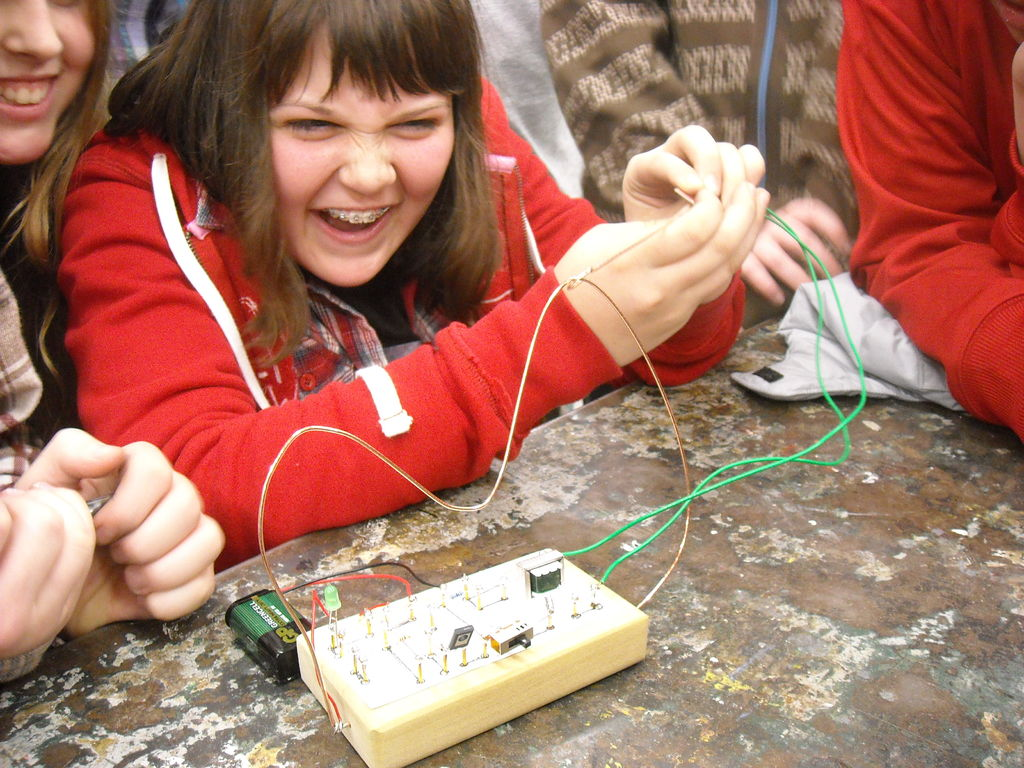
\includegraphics[height=.75\textheight]{Girl}
% \end{frame}



% \section{A vida, o Universo e tudo mais} %%%%%%%

\subsection{Conselhos práticos} %%%%%%%

\begin{frame}{Aprendizado em equipe} % prática
	\center	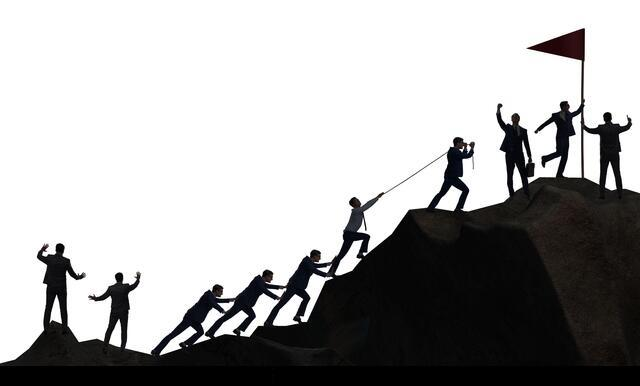
\includegraphics[height=.75\textheight]{climb}
\end{frame}

% \begin{frame}{\insertsubsection} 
% 	\center	
\includegraphics[height=.75\textheight]{figs/duty_calls}
% \end{frame}

% \begin{frame}{\insertsubsection} 
% 	\center	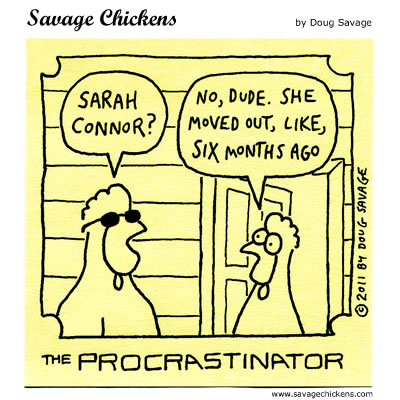
\includegraphics[height=.75\textheight]{figs/chickenprocrastinator}
% \end{frame}

% \begin{frame}{\insertsubsection} 
% 	\center	
\includegraphics[height=.75\textheight]{figs/Procrastination-Dinosaurs-Noahs-Ark-cartoon}
% \end{frame}

% \begin{frame}{\insertsubsection} 
% 	\center	
\includegraphics[height=.75\textheight]{figs/ReverseProcrastination}
% \end{frame}

% \begin{frame}{\insertsubsection} 
%     \center
%     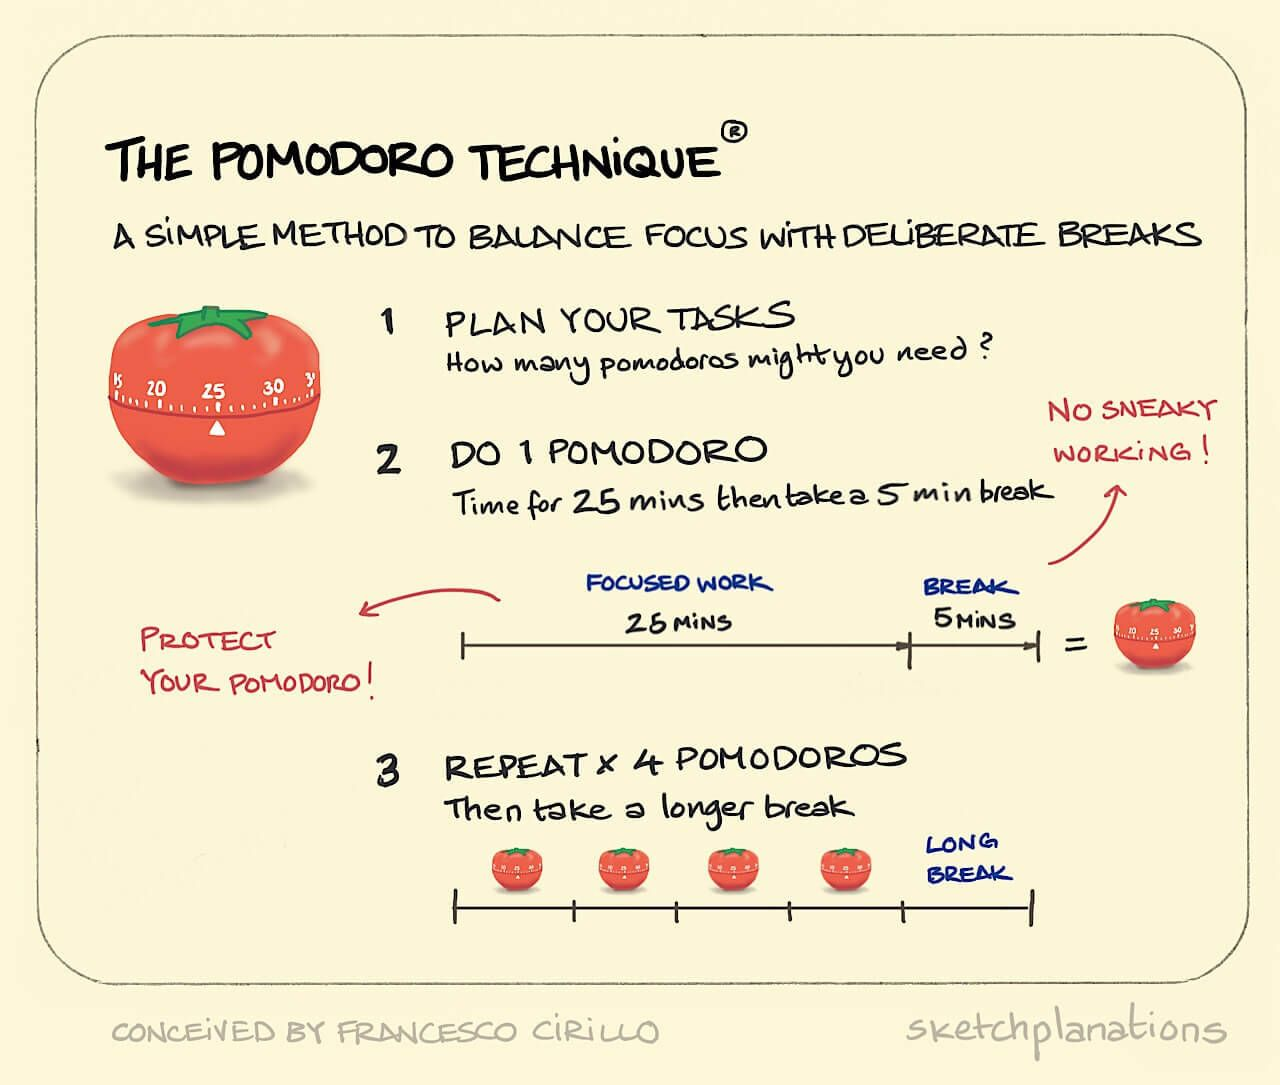
\includegraphics[height=.75\textheight]{figs/pomodoro}
% \end{frame}

\subsection{Sugestões para Leitura} %%%%%%%

\begin{frame}{\insertsubsection} 
    \small 
    \begin{itemize}
        \item \href{https://www.calnewport.com/}{Prof. Cal Newport (Georgetown University) Podcast \& Books}
        \item \href{https://waitbutwhy.com/2013/10/why-procrastinators-procrastinate.html}{Why Procrastinators Procrastinate}
        \item \href{https://www.ted.com/talks/tim_urban_inside_the_mind_of_a_master_procrastinator}{Inside the mind of a master procrastinator}
        \item \href{http://qga.com.br/comportamento/jovem/2013/09/porque-os-jovens-profissionais-da-geracao-y-estao-infelizes}{Porque os jovens profissionais da geração Y estão infelizes}
        \item \href{https://www.amazon.com.br/Talent-Overrated-Separates-World-Class-Performers/dp/1591842948}{Talent Is Overrated:\\What Really Separates World-Class Performers from Everybody Else}
    \end{itemize}
\end{frame}

\begin{frame}
	\titlepage
\end{frame} 

\end{document}